\documentclass[11pt]{article}
\usepackage[margin=1in]{geometry}
\usepackage{amsmath,amssymb}
\usepackage{lmodern}
\usepackage[T1]{fontenc}
\usepackage{enumitem}
\usepackage{microtype}
\usepackage{tikz}
\usetikzlibrary{arrows.meta,angles,quotes,calc,decorations.pathreplacing}

\title{2009 F=ma Exam Review}
\author{Nathan P.}
\date{December 13, 2025}

\begin{document}
\maketitle

\section*{Problem 1}
$Ft=mv$, and don't forget the radical in $v=\sqrt{2gh}$. Also, instead of thinking through the kinematic equations for the final velocity, when something falls just think of the energy result: $v=\sqrt{2gh}$.
Get the pressure by solving for $F$ and dividing by $A$:
\[
A=4\ \text{cm}^2\cdot\frac{1\ \text{m}^2}{(100\ \text{cm})^2}=\frac{4}{100^2}\ \text{m}^2.
\]
Unit conversions.

\section*{Problem 2}
Elastic collisions: exchange $v$ if $m$ is the same. First collision: middle block moving right. Second collision: middle block moving left (middle and left exchange the same $v$). Third collision: middle block back to start, left block moves off.

\section*{Problem 4}
Yes, the net acceleration up is $5g$. However, you must sum the forces on the spaceman to get the normal force between them: $N-mg=m(5g)$, not just $N=m(5g)$. So $N=6mg$.

\section*{Problem 5}
$v_{\text{orb}}=\sqrt{GM/r}$, so $L=mvr=mr\sqrt{GM/r}=m\sqrt{GMr}$. So $L\propto\sqrt r$: larger $r$, larger $L$.
Since $L$ is constant, even though orbit B is elliptical, it will have an $L$ somewhere between A and C, because the orbit's overall size is between theirs.

\section*{Problem 6}
You can use energy or kinematics to get the result: $v^2=v_0^2-2gh$, meaning the speed at height $h$ is independent of the angle.

\section*{Problem 13}
This question isn't trying to be ambiguous. The torque is taken about the fulcrum. Since they're spaced out evenly but have different masses, the fulcrum must be between Lucy and Henry, because Lucy is heavier than Mary, so Henry needs to provide some torque to balance it.
Since the seesaw balances, the torque on the left should equal the torque on the right: $\tau_{\text{Lucy}}=\tau_{\text{Henry}}+\tau_{\text{Mary}}$. Now it's clear that $\tau_{\text{Lucy}}$ is the greatest, because that's the one torque balancing the two others.
Numerically, the fulcrum is at the com, and plugging in numbers indeed shows Lucy has the greatest torque. However, it is best to approach this problem conceptually.

\section*{Problem 14}
\begin{itemize}[leftmargin=*, itemsep=0.25em]
\item A: Linear momentum is not conserved because there are external forces acting on the system during this 20 second interval: tension and gravity.
\item B: Horizontal linear momentum isn't conserved either. Tension (an external force) has a horizontal component.
\item C: Energy isn't conserved because this is an inelastic collision.
\item D: Angular momentum about the peg is also not conserved, because gravity provides an external torque during the long time interval after the collision, changing $L$ about the peg.
\end{itemize}
Overall, when the block-bullet system reaches its peak height, it has zero linear and angular momentum, so they're clearly not conserved.

\section*{Problem 17}
The key concept this question is testing: you're given two different base dimensions, mass and time.
Now just test the answer options for what you can measure with those, and it turns out to be the spring constant, which only depends on mass and time (kg/s$^2$).

\section*{Problem 22}
Period of an orbit of two bodies around their com:
\[
T^2=\frac{4\pi^2}{G(M+m)}d^3.
\]

\section*{Problem 24}
The question is asking for the relationship so that the block will tip before slipping at the critical angle.
We know $\tan\theta_{\text{slip}}=\mu$; now we need a relationship for $\theta_{\text{tip}}$.
When it's tipping, the normal and therefore friction forces pass through that one point. At the critical tipping angle, gravity passes through that point. Through some geometry, we see $\tan\theta_{\text{tip}}=b/a$.
For $\theta_{\text{tip}}$ to happen before ($<$) $\theta_{\text{slip}}$, $\tan\theta_{\text{tip}}<\tan\theta_{\text{slip}}$, so $b/a<\mu$.

\begin{center}
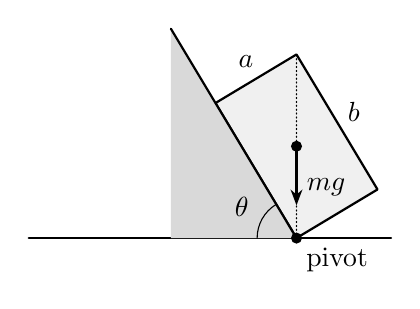
\begin{tikzpicture}[scale=1.0, line cap=round, line join=round, >={Stealth[length=2mm]}]
  % block b (along incline) x a (height), at the tipping angle tan(theta) = b/a
  \coordinate (Z) at (0,0);
  \coordinate (P) at (2.2,0);
  \draw[thick] (-1.2,0) -- (3.4,0);
  \begin{scope}[rotate around={-59.04:(P)}]
    \coordinate (Q) at ($(P)+(-2,0)$);
    \coordinate (Q2) at ($(P)+(-2,1.2)$);
    \coordinate (P2) at ($(P)+(0,1.2)$);
    \coordinate (G) at ($(P)+(-1,0.6)$);
    \coordinate (Top) at ($(P)+(-3.1,0)$);
    \draw[thick, fill=gray!12] (P) -- (Q) -- (Q2) -- (P2) -- cycle;
    \draw[densely dotted] (P) -- (Q2);
    \node at ($(Q)!0.5!(Q2)+(-0.25,0)$) {$a$};
    \node at ($(Q2)!0.5!(P2)+(0,0.25)$) {$b$};
  \end{scope}
  \fill[gray!30] (P) -- (Top) -- (Top |- P) -- cycle;
  \draw[thick] (P) -- (Top);
  \fill (G) circle (2pt);
  \draw[->,thick] (G) -- ++(0,-0.75) node[pos=0.7,right] {$mg$};
  \fill (P) circle (2pt) node[below right] {pivot};
  \pic[draw, "$\theta$", angle radius=5mm, angle eccentricity=1.6] {angle = Top--P--Z};
\end{tikzpicture}
\end{center}

\end{document}
